%!TEX root = ../dissertation.tex
\begin{savequote}[125mm]
    The speaker wants to be understood. %, so he intends to speak in such a way that he will be interpreted in a certain way. 
    In order to judge how he will be interpreted, he uses his [...] starting theory of interpretation. % interpreter’s readiness to interpret along certain lines. %Central to this picture is what the speaker believes is 
%The speaker does not necessarily speak in such a way as to prompt the interpreter to apply this prior theory; he may deliberately dispose the interpreter to modify his prior theory. But the speaker’s view of the interpreter’s prior theory is not irrelevant to what he says, nor to what he means by his words; it is an important part of what he has to go on if he wants to be understood.
As speaker and interpreter talk, their ``prior'' theories become more alike; so do their ``passing'' theories. %The asymptote of agreement and understanding is when passing theories coincide. 
%But the passing theory cannot in general correspond to an interpreter’s linguistic competence. 
Not only does it have its changing list of proper names and gerrymandered vocabulary, but it includes every successful use of any other word or phrase, no matter how far out of the ordinary. 
Every deviation from ordinary usage, as long as it is agreed on for the moment (knowingly deviant, or not, on one, or both, sides), is in the passing theory as a feature of what the words mean on that occasion. 
Such meanings, transient though they may be, are literal.
\qauthor{\vspace{-2em}Donald Davidson, 1986}
\end{savequote}

\chapter{An inferential model of convention-formation}
\graphicspath{{./figures/modeling/}}

Here, we present a probabilistic model of language use under uncertainty, which captures several of the signature properties of convention formation introduced in Chapter 1. 

\section{Adapting to a single partner}
This model belongs to the family of Rational Speech Act (RSA) models, which have been successful in explaining a wide range of linguistic phenomena -- including scalar implicature, adjectival vagueness, overinformativeness, indirect questions, and non-literal language use -- as arising from a process of recursive social reasoning. 
%Most previous applications of RSA have focused on the listener's problem of language comprehension, but the puzzle of conventionalization is primarily a puzzle of speaker production. 

In this framework, an $n$th order pragmatic speaker trying to convey a particular state of affairs $s \in \mathcal{S}$ assuming lexicon $\mathcal{L}$ is assumed to select an utterance $u \in \mathcal{U}$ by trading off its expected informativity (with respect to a rational listener agent) against its cost, usually based on length \cite{GoodmanFrank16_RSATiCS}:
$$S_n(u | s, \mathcal{L}) \propto \exp{\left(\alpha \log L_{n-1}(s | u, \mathcal{L}) - \textrm{cost}(u)\right)}$$
where $\alpha$ is a soft-max optimality parameter controlling the extent to which the speaker maximizes over listener informativity. The listener, in turn, inverts the speaker model to reason about what underlying state $s$ the speaker is trying to convey, given their utterance $u$:
$$L_n(s | u, \mathcal{L}) \propto P(s) S_{n}(u | s, \mathcal{L})$$
\indent This recursion bottoms out in a *literal listener* who directly looks up the meaning of the utterance in the lexicon:
$$L_0(s | u, \mathcal{L}) \propto \mathcal{L}(u, s)\cdot P(s)$$
\indent As in several other recent applications of RSA \cite{GrafEtAl16_BasicLevel}, we use a graded semantics, where utterances are better or worse descriptions of particular referents. For instance, the utterance "dancer" may initially be expected to apply to a photorealistic image of a ballerina ($\mathcal{L}(\textrm{'dancer'}, \textit{ballerina}) = 0.99$) more than an abstract image of one ($\mathcal{L}(\textrm{'dancer'}, \textit{abstract ballerina}) =0.6$), but apply to both better than a non-category member like an image of a dog ($\mathcal{L}(\textrm{'dancer'}, \textit{dog}) = 0.05$).

Our approach to convention-formation begins with the additional assumption of \emph{lexical uncertainty} \cite{SmithGoodmanFrank13_RecursivePragmaticReasoningNIPS,BergenLevyGoodman16_LexicalUncertainty}. 
In other words, we assume that instead of having perfect knowledge of $\mathcal{L}$, the listener has uncertainty over the exact meanings of lexical items in the current context (i.e. it is initially unclear which of the ambiguous tangram shapes "the dancer" might refer to). They begin with some prior $P(\mathcal{L})$ about the identity their partner's true lexicon, which may be initially biased toward certain meanings. By conditioning on repeated observations of their partner's behavior, they use Bayes rule to infer this true lexicon:
$$P_{L_n}(\mathcal{L} | d) \propto P(\mathcal{L})\prod_i S_n(s_i|u_i, \mathcal{L})$$
where $d = \{s_i, u_i\}$ is a set of observations of $s_i$ and $u_i$ coming from previous exchanges\footnote{There is a broader debate over the timescales at which lexicons and lexicon learning mechanisms operate; here, we assume a discourse-level structure to the lexicon, where there is uncertainty over how words are used \emph{in the given conversation, by the current partner}. See \cite{FrankGoodmanTenenbaum09_Wurwur} for a related approach at the scale of cross-situational word learning.}. 
The listener marginalizes over this posterior when interpreting the speaker's utterance:
$$L_n(s | u, d) \propto \sum_\mathcal{L}P_{L_n}(\mathcal{L}|d)L_n(s|u,\mathcal{L})$$
The speaker, in turn, considers what utterances would be most informative for such a listener:
$$S_n(u | s, d) \propto \exp( \alpha\log\left(\sum_{\mathcal{L}} P_{S_n}(\mathcal{L} | d) L_{n-1}(s | u, \mathcal{L})\right) - \textrm{cost}(u) )$$
where the posterior over lexica $P_{S_n}(\mathcal{L} | d)$, uses the listener likelihood $L_{n-1}$. For the purposes of this paper, we fix the depth of recursion at $n = 2$.
This model is implemented in the probabilistic programming language WebPPL \cite{GoodmanStuhlmuller14_DIPPL}. \footnote{All results can be reproduced running our code in the browser at \url{http://forestdb.org/models/conventions.html}}. 

\subsection{Model Results}

\begin{figure}
\centering
    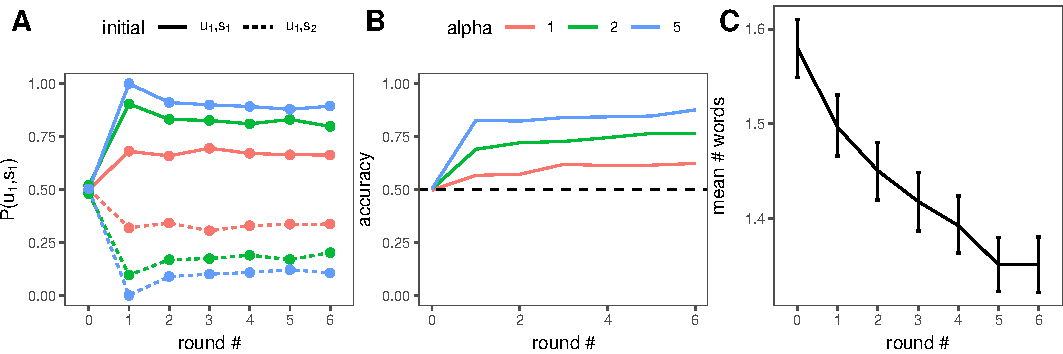
\includegraphics[scale=.8]{modelResults.pdf}
  \caption{Schematic of model}
  \label{fig:task1model}
\end{figure}

Following \cite{SmithGoodmanFrank13_RecursivePragmaticReasoningNIPS}, we begin by showing how a random initial choice is taken to be evidence for a particular lexicon and becomes the base for successful communication even though neither party knows its meaning at the outset.
Consider an environment with two abstract shapes ($\{s_1, s_2\}$), where the speaker must choose between two utterances ($\{u_1, u_2\}$) incurring equal cost. 
Their prior $P(\mathcal{L})$ over the meaning of each utterance is given by a Beta distribution\footnote{In our implementation, we enumerate over coarse-grained bins; preliminary experiments using variational inference on the full continuous distribution give similar results}, so on the first round both utterances are equally likely to apply to either shape. 
If the speaker was trying to get their partner to pick $s_1$, then, since each utterance is equally (un)informative, they would randomly sample one (say, $u_1$), and observe the listener's selection of a shape (say, $s_1$). 
On the next round, the speaker uses the observed pair $\{u_1, s_1\}$ to update their beliefs about their partner's true lexicon, uses these beliefs to generate a new utterance, and so on. 
To examine expected dynamics over multiple rounds, we forward sample many possible trajectories.

We observe several important qualitative effects in our simulations. 
First, the fact that a knowledgeable listener responds to utterance $u$ with $s$ provides evidence for lexicons in which $u$ is a good fit for $s$, hence the likelihood of the speaker using $u$ to refer to $s$ increases on subsequent rounds (see Fig.\ref{fig:modelResults}A). 
In other words, the initial symmetry between the meanings can be broken by initial random choices, leading to completely *arbitrary but stable mappings* in future rounds. Second, because the listener is also learning the lexicon from these observations under the same set of assumptions, they converge on a shared set of meanings; hence, expected *accuracy* rises on future rounds (see Fig. \ref{fig:modelResults}B). Third, because one's partner is assumed to be pragmatic, agents can also learn about *unheard* utterances. Observing $d = \{u_1, s_1\}$ also provides evidence that $u_2$ is *not* a good fit for $s_1$ by Gricean maxims: if $u_2$ were a better fit for $s_1$, the speaker would have used it instead \cite{Grice75_LogicConversation}. Finally, *failed references* lead to conventions just as effectively as successful references: if the speaker intends $s_1$ and says $u_1$, but then the listener incorrectly picks $s_2$, the speaker will take this as evidence that $u_1$ actually means $s_2$ in their partner's lexicon and become increasingly likely to use it that way on subsequent rounds.

Finally, we show how our model explains reduction of utterance length over multiple interactions. For utterances to be reduced, of course, they must vary in length. Motivated by our empirical observation that meaningful clauses are the primary unit of reduction, we extend our grammar to include *conjunctions*. This is one of the simplest ways to constructing longer utterances compositionally from lexical primitives, using the product rule:
$$\mathcal{L}(u_i \textrm{ and } u_j, o) = \mathcal{L}(u_i, o) \times \mathcal{L}(u_j, o)$$
\indent Analogous to our tangram stimuli, which have many ambiguous features and figurative perspectives that may be evoked in speaker descriptions, we consider a simplified scenario where speakers can refer to two different features of the two objects $\{o_1, o_2\}$. The speaker has four primitive words at their disposal -- two words for shape ($\{u_{s1}, u_{s2}\}$) and two for color $\{u_{c1}, u_{c2}\}$ -- and has uncertainty over the initial meanings of all four.

While we established in the previous section that conventions can emerge over a reference game in the complete absence of initial preferences, players often bring such preferences to the table. A player who hears 'ice skater' on the first round of our tangrams task is more likely to select some objects more than others, even though they still have some uncertainty over its meaning in the context. To show that our model can accommodate this fact, we allow the speaker's initial prior meanings to be slightly biased. $u_{s1}$ and $u_{c1}$ are more likely to mean $o_1$; $u_{s2}$ and $u_{c2}$ are more likely to mean $o_2$.

We ran 1000 forward samples of 6 rounds of speaker-listener interaction, and averaged over the utterance length at each round \footnote{In our simulations, we used $\alpha = 10$ and found the basic reduction effect over a range of different biases}. Our results are shown in Figure \ref{fig:modelResults}C: the expected utterance length decreases systematically over each round. To illustrate in more detail how this dynamic is driven by an initial rational preference for redundancy relaxing as reference becomes more reliable, we walk step-by-step through a single trajectory. 

Consider a speaker who wants to refer to object $o_1$. They believe their knowledgeable partner is slightly more likely to interpret their language using a lexicon in which $u_{s1}$ and $u_{c1}$ apply to this object, due to their initial bias. However, there is still a reasonable chance that one or the other alone actually refers strongly to $o_2$ in the true lexicon. Thus, it is useful to produce the conjunction "$u_{s1}$ and $u_{c1}$" to hedge against this possibility, despite its higher cost. Upon observing the listener's response (say, $o_1$), the evidence is indeterminate about the separate meanings of $u_{s1}$ and $u_{c1}$ but both become increasingly likely to refer to $o_1$. In the trade-off between informativity and cost, the shorter utterances remain probable options. Once the speaker chooses one of them, the symmetry collapses and that utterance remains most probable in future rounds. In this way, meaningful sub-phrases are omitted over time as the speaker becomes more confident about the true lexicon. 

\section{Partner-specificity and generalization: introducing hierarchical structure into lexical inference}

Hierarchical Bayesian models have been key to quantitatively explaining how the human mind solves difficult inductive problems in domains like causal learning and concept learning where idiosyncratic particulars of instances must be jointly inferred with knowledge that is shared across instances \shortcite{tenenbaum_how_2011}.
For instance, the concept of a ``dog'' abstracts away from our experiences with different instances of dogs across a lifetime, and provides stable expectations about the properties of a new instance -- four legs, wagging tail, barking noises.

%More than the relatively fixed, biological concept of a dog, though, language can be seen as a moving target. The only data we use to ground our learning is produced by other agents who are in the same position as we are, and our only goal is to coordinate on the same meanings in context. This is the sense in which the meanings we learn are conventional. 
However, extensive experience with a particular dog \emph{Fido} reveals idiosyncratic properties, like the pattern of spots on his coat.
This example from concept learning can be adapted as a novel perspective on how conventions work: accumulated knowledge about linguistic conventions in one's community provides stable communicative ``priors'' that guide how we approach new partners, but the language we use to talk with a family member or close collaborator may deviate considerably from the usage predicted by population-level conventions.

Hierarchical Bayesian models thus provide a formal method for both smoothly integrating population-level expectations with partner-specific ones, and also appropriately \emph{updating} population-level knowledge through additional partner-specific observations. 

We begin by proposing a hierarchical Bayesian model of convention formation \cite{GelmanEtAl14_BDA,TenenbaumKempGriffithsGoodman11_Grow_a_Mind_Science} that provides a useful mathematical and conceptual framework for addressing these challenges. Hierarchical models have been key to explaining how the human mind solves difficult inductive problems in domain like causal learning \cite{KempGoodmanTenenbaum10_LearningToLearn,GoodmanUllmanTenenbaum11_TheoryOfCausality} and concept learning \cite{KempPerforsTenenbaum07_HBM} where abstract, shared properties must be jointly inferred with idiosyncratic particulars of instances. More than the relatively fixed, biological concept of a dog, though, language is a moving target. The only data we use to ground our learning is produced by other agents who are in the same position as we are, and our only goal is to coordinate on the same meanings in context \cite{HassonGhazanfar___Keysers12BrainToBrain}. This is the sense in which the meanings we learn are conventional. This \emph{social grounding} is precisely what gives rise to the fascinating idiosyncracies of local convention formation.

We begin by defining a lexicon as a function $$\mathcal{L}_i: (w, o) \rightarrow [0,1]$$ assigning any word-object pair a real-valued meaning in the unit interval \cite{GrafEtAl16_BasicLevel}\footnote{
We mostly have nouns (\emph{poodle, animal, John}) and property adjectives (\emph{blue, squiggly, delicious}) in mind here, which can be assigned direct semantic meanings. How tricker cases like relational modifiers (\emph{some, barely, former}) are represented in the mental lexicon and how to build a fully compositional semantics from them is a topic of ongoing work in formal semantics, though see \citeA{Yildirim16_TalkerSpecificityQuantifiers} for a study exploring how these too can adapt in partner-specific ways over repeated interaction.
}. There are \emph{many} potential ways this function could be represented in the mind at the algorithmic level. It could be derived from a store of exemplars, a set of independent prototypes for each word, a neural network embedding words and objects in a vector space, and so on \cite<see>[for a recent review of candidates]{JonesEtAl15_SemanticMemory}.

Just as our concept of a dog, built up over many individual experiences across a lifetime, provides stable expectations about the properties of a new instance -- four legs, wagging tail, barking noises -- our accumulated lexical knowledge provides stable communicative expectations. 
This knowledge is represented by a `overhypothesis' or shared lexical representation $\Theta_0$, which parameterizes the prior expectations about any individual partner's lexicon: $P(\mathcal{L}_i | \Theta_0)$. 

For the conceptual purposes of this paper, it is not important exactly what form this distribution takes, or what initial prior over the overhypothesis $P(\Theta_0)$ could in principle guide early language learning
\footnote{
For simplicity, we could assume $\Theta_0$ is an $\mathcal{W} \times \mathcal{O} \times 2$ tensor containing values $(\alpha_{(w,o)}, \beta_{(w,o)})$ for every entry $(w,o)$ in the lexicon $\mathcal{L}_i$. This would factor the lexical prior $P(\mathcal{L}_i | \Theta_0)$ into independent Beta distributions over intervals $[0,1]$. It would then be straightforward to place an uninformative prior $P(\Theta_0)$ over that tensor which does not overwhelm the likelihood \cite<see>[p. 110, for some reasonable choices]{GelmanEtAl14_BDA}. More generally, we could allow for arbitrarily complex dependencies between entries of the lexicon by using a Bayesian neural network with weight tensor $\Theta_0$.% that takes word-object pairs $(w,o)$ as input. 
}. It only matters that this knowledge is hierarchical: we expect all members of our language community to share some commonality in what they mean by things. 

Now that we have defined a hierarchical likelihood on lexical beliefs, we must say how we \emph{learn} partner-specific models. Just as years of living with your beloved Fido reveals properties which deviate from your general dog concept -- patches of hair missing from his legs, an odd squeaking noise he makes when excited -- the language we use to talk with a family member or close collaborator may deviate considerably from the usage predicted by global conventions. In other words, our beliefs about a particular partner's lexicon $\mathcal{L}_i$ are formed by integrating our abstract lexical knowledge $\Theta_0$ with particular  observations $D_i$ of that particular individual:
$$%\begin{array}{rcl}
P(\mathcal{L}_i | D_i)  \propto \int_{\Theta_0}P(\mathcal{L}_i | D_i,  \Theta_0) P(\Theta_0 | D_i) 
%                     & = & \mathbb{E}_{\Theta_0}[P(\mathcal{L}_i | \Theta_0, D_i)] 
%\end{array}
$$
where the posteriors in the integral can be computed using Bayes rule:
$$
P(\mathcal{L}_i | D_i, \Theta_0) \propto P(D_i | \mathcal{L}_i, \Theta_0) P(\mathcal{L}_i | \Theta_0)
$$
While this holds when we only have observations from a single speaker, note that our posterior beliefs about $\Theta_0$ are in fact informed by observations from \emph{all} speakers: $D = \bigcup_{i=1}^k D_i$. For  adult language users who have observed innumerable uses of language over their lifetimes, the contribution of a new data point to the overhypothesis $P(\Theta_0 | D)$ should be negligible; the contribution to a partner-specific model, however, can be quite strong. 

Finally, to fully specify our model and compute our partner-specific lexical posterior $P(\mathcal{L}_i, D_i, \Theta_0)$, we must link our beliefs about a partner's lexica to their actual behavior with a likelihood function $P(D_i | \mathcal{L}_i, \Theta_0)$. This is naturally supplied by the Rational Speech Act framework \cite{FrankGoodman12_PragmaticReasoningLanguageGames,GoodmanFrank16_RSATiCS,BergenLevyGoodman16_LexicalUncertainty,SmithGoodmanFrank13_RecursivePragmaticReasoningNIPS}: we assume speakers produce utterances that are parsimonious yet informative in context with respect to their lexicon, and listeners interpret utterances by inverting a speaker model. Because we expect our partner to use language rationally given some lexicon, the utterance they choose to refer to some object will be probable under some lexica and highly improbable under others. In this way, a particular agent's language use is a cue to their particular lexicon. We omit mathematical details here due to the conceptual nature of the article, but a full account of the non-hierarchical version of this model can be found in \citeA{HawkinsFrankGoodman17_ConventionFormation}.

In summary, our hierarchical model formalizes the intuition that global conventions are learned and generalized over many extended interactions with many different people across a lifetime, and that this shared semantic prototype is the backbone supporting rapid learning for new partners and situations. 

\subsection{From grant (maybe cleaner than above?)}
This model will extend the non-hierarchical Bayesian model of \emph{partner-specific} adaptation I developed in my dissertation work \shortcite{hawkins_convention-formation_2017, hawkins_emerging_abstractions_2018} to multiple partners, thus providing the first opportunity to test how collective patterns emerge from rich, repeated interactions with known partners in a community. 
Here I sketch the ``ideal'' mathematical form of the proposed model, leaving implementational details for the following section.

\begin{figure}
\centering
    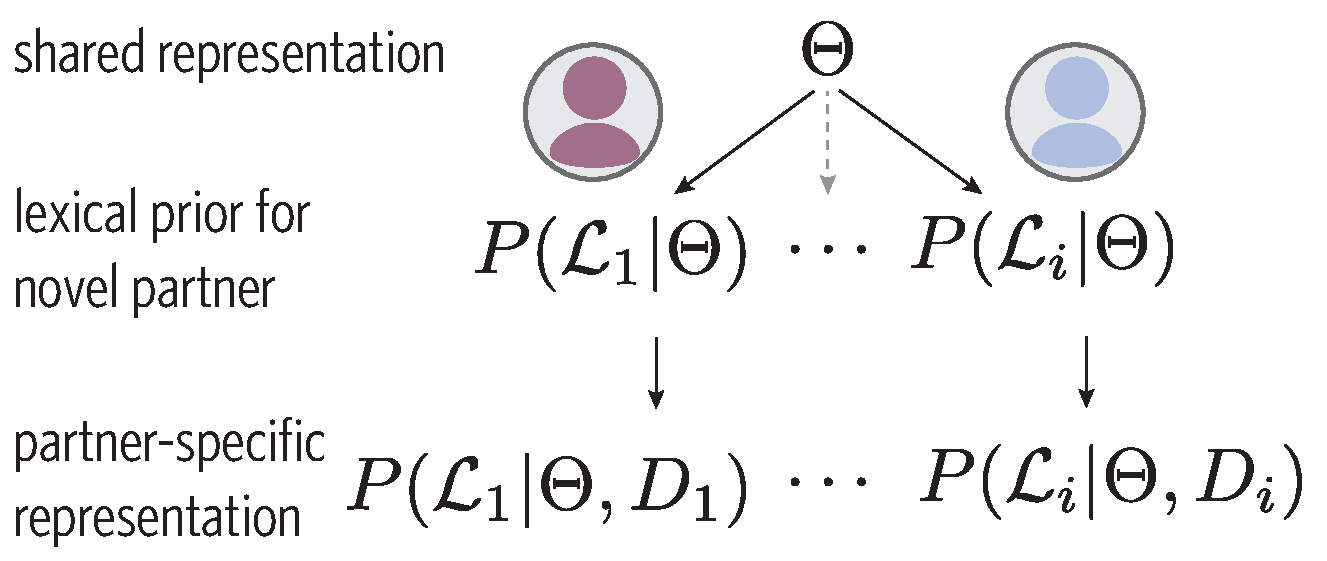
\includegraphics[scale=.45]{task1_model.pdf}
  \caption{Schematic of model}
  \label{fig:task1model}
\end{figure}
At the core of any model of referential communication is the notion of a \emph{lexicon} giving the meanings of the tokens in the language. 
We define the lexicon as a function $\mathcal{L}: (w_n, o_m) \rightarrow \mathbb{R}$, assigning any word-object pair a real-valued meaning according to how well the word $w_n$ applies to the object $o_m$. 
This is a continuous generalization of classic truth-conditional semantics \shortcite{graf_animal_2016}. 
We view the lexicon not as a lookup table or a static logical form untouched after childhood, but as a dynamic, parameterized representation that is constantly being updated.
 %\footnote{
%We mostly have nouns (\emph{poodle, animal, John}) and property adjectives (\emph{blue, squiggly, delicious}) in mind here, which can be assigned direct semantic meanings. How tricker cases like relational modifiers (\emph{some, barely, former}) are represented in the mental lexicon and how to build a fully compositional semantics from them is a topic of ongoing work in formal semantics, though see \citeA{Yildirim16_TalkerSpecificityQuantifiers} for a study exploring how these too can adapt in partner-specific ways over repeated interaction.
%}. 
%There are \emph{many} potential ways this function could be represented in the mind at the algorithmic level. It could be derived from a store of exemplars, a set of independent prototypes for each word, a neural network embedding words and objects in a vector space, and so on \cite<see>[for a recent review of candidates]{JonesEtAl15_SemanticMemory}.
At the highest level of the hierarchical lexical representation is a \emph{community-level} variable $\Theta$ parameterizing the agent's prior expectations for the likely lexicon $\mathcal{L}_i$ used by a novel community member $i$: $P(\mathcal{L}_i | \Theta)$. 
%For simple domains where the vocabulary and number of objects is small, $\Theta_0$ could simply be a $$n\times m$$ a $\times$ real-valued matrix where $n$ is the vocabulary size and $m$ is the number of objects, but for more natural tasks, it is 
%For the conceptual purposes of this paper, it is not important exactly what form this distribution takes, or what initial prior over the overhypothesis $P(\Theta_0)$ could in principle guide early language learning
%\footnote{
%For simplicity, we could assume $\Theta_0$ is an $\mathcal{W} \times \mathcal{O} \times 2$ tensor containing values $(\alpha_{(w,o)}, \beta_{(w,o)})$ for every entry $(w,o)$ in the lexicon $\mathcal{L}_i$. This would factor the lexical prior $P(\mathcal{L}_i | \Theta_0)$ into independent Beta distributions over intervals $[0,1]$. It would then be straightforward to place an uninformative prior $P(\Theta_0)$ over that tensor which does not overwhelm the likelihood \cite<see>[p. 110, for some reasonable choices]{gelman2006data}. More generally, we could allow for arbitrarily complex dependencies between entries of the lexicon by using a Bayesian neural network with weight tensor $\Theta_0$.% that takes word-object pairs $(w,o)$ as input. 
%}. It only matters that this knowledge is hierarchical: we expect all members of our language community to share some commonality in what they mean by things. 

Given observations $D_i$ from interactions with that particular individual---concretely, utterances and responses in a reference game---their \emph{partner-specific} model can be rapidly updated using Bayes rule:
$%\begin{array}{rcl}
P(\mathcal{L}_i | D_i, \Theta)  \propto P(D_i | \mathcal{L}_i) P(\mathcal{L}_i | \Theta)P(\Theta)
%                     & = & \mathbb{E}_{\Theta_0}[P(\mathcal{L}_i | \Theta_0, D_i)] 
%\end{array}
$.
%While this holds when we only have observations from a single speaker, note that our posterior beliefs about $\Theta_0$ are in fact informed by observations from \emph{all} speakers: $D = \bigcup_{i=1}^k D_i$. For  adult language users who have observed innumerable uses of language over their lifetimes, the contribution of a new data point to the overhypothesis $P(\Theta_0 | D)$ should be negligible; the contribution to a partner-specific model, however, can be quite strong. 
Additionally, because the partner-specific model depends on $\Theta$, Bayesian inference allows new data to systematically inform the shared, population-level representation as well (Fig. \ref{fig:task1model}).
Critically for predictions about generalization, new language data (i.e. particular ways of referring to the tangram shapes) may at first be more parsimoniously explained as an idiosyncratic property of a particular partner's lexicon, or ``idiolect''. 
If two or three partners all happen to use the same language, however, it starts to become more likely that a novel partner will share it as well (this transfer is sometimes referred to as ``sharing of statistical strength.'')
This formalizes the intuition from the behavioral predictions.


%In summary, our proposed hierarchical Bayesian model formalizes the intuition that global conventions are learned and generalized over many extended interactions with many different people across a lifetime, and that this shared semantic prototype is the backbone supporting rapid learning for new partners and situations. 

\subsection{Model implementation}
To implement this model, we must specify (1) the parameterization of the lexicon, (2) the linking function (i.e. likelihood function) between parameter values and observed language behavior, and (3) an algorithm to perform inference.
First, for small finite domains with $N$ words and $M$ objects, a natural parameterization of the lexicon is an $N\times M$ matrix where each cell is the value of a lexical entry, as I previously used in my dissertation work \cite{hawkins_emerging_abstractions_2018}. 
In Objective 3, we will use a neural network to extend this efficiently to arbitrarily large spaces.
Second, a natural linking hypothesis to behavior is provided by the Rational Speech Act framework, which I have helped developed throughout my dissertation work \shortcite{hawkins_why_2015,goodman_pragmatic_2016,bergen_pragmatic_2016}. 
In this framework, speakers produce utterances that are parsimonious yet informative in context with respect to their lexicon, and listeners interpret utterances by inverting a speaker model. 
Because agents expect their partner to use language rationally given some lexicon $\mathcal{L}_i$, their language use is therefore a probabilistic cue to their lexicon.
Third, we will perform inference in this model using Hamiltonian Monte Carlo (HMC) which uses gradient information to quickly converge on samples from the posterior; if HMC fails, we will use mean-field variational inference (VI), which uses stochastic gradient descent to minimize the divergence between the true posterior and a parameterized approximating family of Gaussians.

